\subsection{Parallelism of Pipeline Join}\label{sec:experiments_join}
This section tests the speedup of using multiple cores. The speedup is calculated by the time using a single core divided by the time using multiple cores for a specific query. 
%The purpose of this experiment is to study the CPU parallelism of SeqStar's pipeline join.
We choose two of the most time-consuming queries $q_6$ and $q_8$ for the study.
%We use speedup to measure the parallelization effect, which is the elapsed time of the single thread join over that of the multi-threaded execution.

Figure~\ref{img:exp_scalability} shows the speedup of SeqStar's pipeline join by varying the number of threads from 1 to 32.
SeqStar has a nearly linear speedup due to the independence of loops in our pipeline join (\S\ref{sec:match_join}).
Noticeably, SeqStar achieved almost optimal speedup within 8 threads.
Specifically, the speedup of BS $q_6$ is 7.6 using 8 threads and the speedup of GO $q_6$ is 6.7.
\begin{figure}[ht]
  \centering
  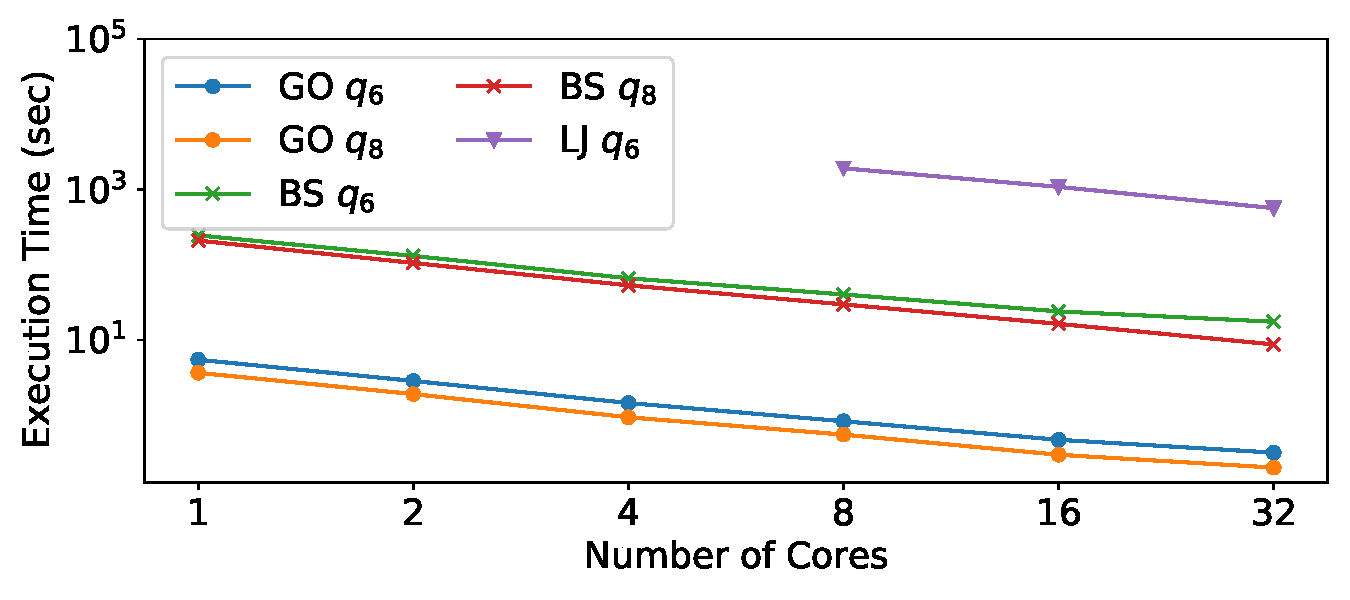
\includegraphics[width=0.5\textwidth]{img/exp_scalability.pdf}
  \caption{Scalability of Pipeline Join.}\label{img:exp_scalability}
\end{figure}

\subsection{Performance of Predicate Pushdown}
In order to understand the benefits of predicate pushdown,
we ran four of the most time-consuming queries $q_4$, $q_5$, $q_6$ and $q_8$ with the following WHERE clause:
\begin{Verbatim}[fontsize=\small]
  WHERE u1 % 5 = 0 AND u2 % u1 = 5
\end{Verbatim}
The analyzer of SeqStar will analyze the WHERE clause and obtain:
(1) a vertex-constraint $u_1 \bmod 5 = 0$ and (2) an edge-constraint $u_2 \bmod u_1 = 5$ (\S\ref{sec:match_optimize}).
These constraints can be applied during the star matching process.

Table~\ref{tab:pushdown_lj} and Table~\ref{tab:pushdown_ok} illustrate the effects of predicate pushdown on LJ and OK\@.
$T$ is the execution time with the optimization, i.e., the constraints have to be checked after the graph isomorphism result is obtained.
$T_{OPT}$ is the execution time with predicate pushdown.
$\#R$ is the result size (number of rows) for the queries without the WHERE clause and $\#R_{OPT}$ is the number of rows with WHERE clause applied.

Because of the vertex-constraint $u_1 \bmod 5 = 0$,
the \textsc{VertexIter} can skip invalid vertices whenever possible.
When scanning the \textsc{NeighborIter}s,
the edge-constraint $u_2 \bmod u_1 = 5$ is performed to filter out unnecessary matchings.
The star matching time reduces is reduced by $20\%$ --- $62\%$ in these experiments,
and up to $8 \times 10^5 \times$ of unnecessary results are avoided.
As a result, the total execution time obtains a speedup larger than 525$\times$.
\begin{table}
  \caption{Performance of Predicate Pushdown (LJ)}\label{tab:pushdown_lj}
  \begin{tabular}{lrrrrrr}
    \toprule
    $q$ & \parbox{5mm}{$T$ (sec)} & \parbox{5mm}{$T_{OPT}$ (sec)} & $\frac{T}{T_{OPT}}$ & $\#R$ & $\#R_{OPT}$ & $\frac{\#R}{\#R_{OPT}}$ \\
    \midrule
    4 &   944 &        11 &       89 &   $1.0 \times 10^{12}$ &   $6.6 \times 10^7$ &     15376 \\
    5 & >2100 &         4 &     >525 &  $3.2 \times 10^{13}$  &   $6.7 \times 10^8$ &     47520 \\
    6 &   571 &        24 &       24 &   $6.2 \times 10^{11}$ &   $1.6 \times 10^8$ &      3774 \\
    8 &  1513 &        24 &       63 &   $1.7 \times 10^{13}$ &    $2.0 \times 10^9$ &      8512 \\
    \bottomrule
  \end{tabular}
\end{table}

\begin{table}
  \caption{Performance of Predicate Pushdown (OK)}\label{tab:pushdown_ok}
  \begin{tabular}{lrrrrrr}
    \toprule
    $q$ & \parbox{5mm}{$T$ (sec)} & \parbox{5mm}{$T_{OPT}$ (sec)} & $\frac{T}{T_{OPT}}$ & $\#R$ & $\#R_{OPT}$ & $\frac{\#R}{\#R_{OPT}}$ \\
    \midrule
    4 & >2100 &        65 &      >32 &  $5.6 \times 10^{13}$ &   $1.7 \times 10^{10}$ &      3110 \\
    5 & >2100 &         7 &     >300 &  $3.8 \times 10^{14}$ &     $4.6 \times 10^8$ &     813540 \\
    6 &  1399 &        38 &       37 &  $4.4 \times 10^{10}$ &     $8.3 \times 10^5$ &      53035 \\
    8 &  1347 &        36 &       38 &  $1.4 \times 10^{13}$ &     $6.1 \times 10^8$ &      22609 \\
    \bottomrule
  \end{tabular}
\end{table}
